% !TEX root = ../main.tex
\chapter{Testing}
\label{Testing}

The final product of this project should be a realistic simulation of a Decentralised Community Energy System. To produce the simulation, each of the following features will be tested to ensure they work individually and together:

\begin{itemize}
\item A network of Agents able to trade electricity with each other.
\item Agents are able to utilise energy. The amount of energy utilised can be pre-determined manually by an operator of the simulation or automatically with an algorithm.
\item Agents are able to generate an amount of energy corresponding to a pre-allocated fixed output, or an amount based on their assigned Generation Profiles.
\item Each Agent is able to utilise and generate electricity at the same time.
\end{itemize}

Due to time constraints, unit testing was not implemented. A series of tests was done manually by exporting the data using Excel to prove that the simulator was working as inteneded. The testing has been outlined in the sections below. Each of the tests below has been conducted for the following simulation cases:

\begin{itemize}
	\item 1 Supervisor, 1 Virtual Agent and 1 Agent
	\item 1 Supervisor, 2 Virtual Agent and 2 Agents (Each Virtual Agent connected to 1 Agent)
	\item 1 Supervisor, 2 Virtual Agents and 4 Agents (Each Virtual Agent connected to 2 Agents)
	\item 1 Supervisor, 5 Virtual Agents and 25 Agents (Each Virtual Agent connected to 5 Agents)
\end{itemize}

\section*{Contribution to Pool} % (fold)
To test that Agents are able to contribute to the Common Pool, the individual Demand and Generation request of each Agent was recorded in a CSV file. The allocations in the CSV file was summed and compared to that of the computed Global Demand and Generation request.

An example can be seen in \ref{fig:test1} of testing the contribution of 25 Agents during hour 23 of a simulation

\begin{figure}[h!]
	\centering
	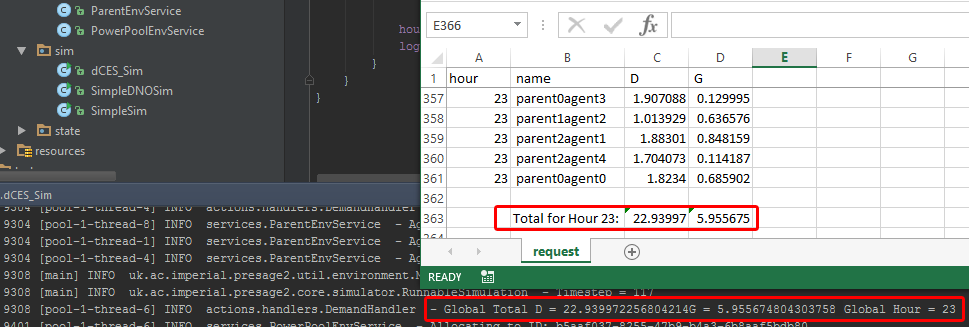
\includegraphics[scale=0.4]{Images/test-contribution.png}
	\caption{Testing the contribution at hour 23 of the simulation for 25 Agents}
	\label{fig:test1}
\end{figure}

\section*{Correct Allocation}
When the global aggregated Generation requests exceed the global aggregated Demand requests, all Agents are expected to receive their requests. Globally, Generation is curtailed to not exceed total Demand Request. Generation is curtailed proportionally for everyone. In this case, we should expect all Agents to be allocated less Generation than they have requested, and all Agents to be allocated their Demand requests. \\

An example of this test can be seen in \ref{fig:test2}. \\

\begin{figure}[h!]
	\centering
	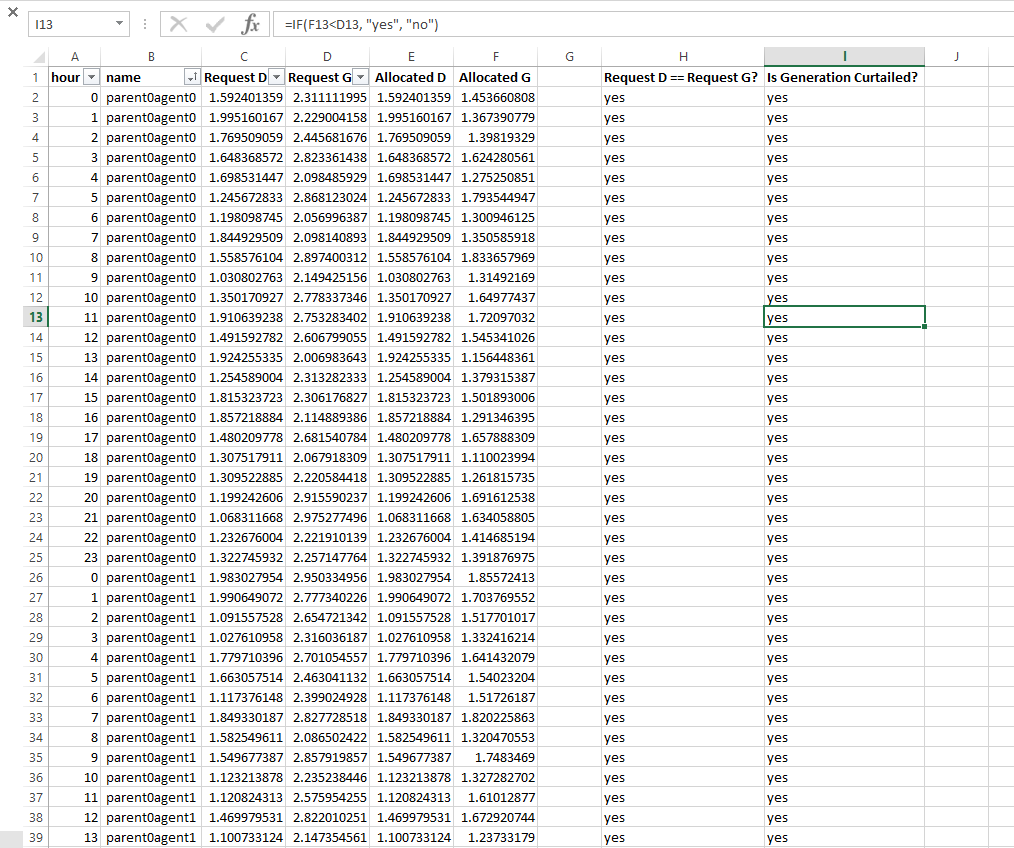
\includegraphics[scale=0.4]{Images/test-allocation1.png}
	\caption{Testing the allocation of 25 Agents when total Generation Request Exceeds total Demand Request}
	\label{fig:test2}
\end{figure}

When the global aggregated Demand request exceed the global Demand request, the fair allocation method will need to be used. For testing this, we need to ensure the following:

\begin{itemize}
	\item Allocated Demand is equal to Allocated Generation
	\item Allocated Generation is equal to Generation request
	\item Allocation proportion is correct
	\item Borda ranking is correct for each of the canons
	\item Borda voting by the Agents are correct
	\item Borda voting is taken into consideration in the next round
\end{itemize}

To be continued...

% section section_name (end)
%If data is available for the potential customers in Rugaragara, the simulation could be used in %conjunction with the feasibility study